%\section{Background on Refresh}
%DRAM needs to be refreshed periodically to prevent data loss. According to JEDEC \cite{JEDEC:ddr3}, 8192 all-bank auto-refresh ({\tt REF}) commands are sent to all DRAM devices in a rank within one retention time interval ({\tt Tret}), also called as one refresh window ({\tt tREFW}) \cite{TC15:refresh, ISCA13:ddr4, HPCA14:parallelrefresh}, typically 64ms for DDR3/4. The gap between two {\tt REF} commands is termed as refresh interval ({\tt tREFI}), whose typical value is 7.8$\mu$s, i.e. 64ms/8192.If a DRAM device has more than 8192 rows, rows are grouped into 8192 {\bf refresh bins}. One {\tt REF} command is used to refresh multiple rows in a bin. An internal counter in each DRAM device tracks the designated rows to be refreshed upon receiving {\tt REF}. The refresh operation takes {\tt tRFC} to complete, which proportionally depends on the number of rows in the bin.

%The refresh rate of one bin is determined by the leakiest cell in the bin. Liu~{\em et~al.} \cite{ISCA12:raidr} reported that fewer than 1000 cells require a refresh window shorter than 256ms in a 32GB DRAM main memory. Given that the majority of rows have retention time longer than 64ms, it is beneficial to enable multi-rate refresh, i.e., different bins are refreshed at different rates. The weakest cell in one bin determines the refresh rate of the bin. For discussion purpose, a DRAM cell/row/bin that is refreshed at 256ms is referred to as a \underline{256ms-cell}/\underline{row}/\underline{bin}, respectively.

%We adopt the {\em flexible auto-refresh} mechanism from \cite{ISCA15:reflex} to support multi-rate refresh, i.e., 8192 refresh commands are sent every 64ms --- one for each bin. If a bin needs to be refreshed every 256ms,  {\em flexible auto-refresh} sends four {\tt REF} commands in 256ms to this bin. However, only one is a real refresh while the other three are dummy ones that only increment the refresh counter. 

%While the bin counter is maintained in the memory controller and incremented sequentially, the actual row addresses (responding to each bin-refresh command) are generated internally inside DDR3/4 devices \cite{JEDEC:ddr3,JEDEC:ddr4}. This mapping may be non-linear because of vendor's full flexibility to implement the refresh.Recent studies \cite{ISCA15:reflex, ISCA14:disturbance} assume this mapping can be made known to the memory controller. We make the same assumption in this paper.
%We assume that the memory controller knows the mapping between bin address and row address, the same as that in \cite{ISCA15:reflex}, and similar to \cite{ISCA14:disturbance}.

\section{Motivation of Partial Restore}
Due to intrinsic leakage, the voltage level of a DRAM cell reduces monotonically after a full restore. The solid curve in Figure \ref{fig:partial} illustrates the voltage decay of an untouched cell (i.e., not accessed) within one refresh window, commonly 64ms. Stored data is safe as long as the voltage remains above V$_{min}$ (0.73V$_{dd}$
\footnote{Value is calculated on basis of charge sharing expression \cite{BOOK13:sharing} and offset noise \cite{JSSC02:sense}, details can be found in \cite{HPCA16:twr}.}
 here)  before the next refresh. If a read or write access occurs, the post-access restore operation fully charges the cell, as shown in the figure. However, the full charge is often unnecessary if the access is {\em close in time} to the next refresh, which will fully restore the cell anyway.

\begin{figure}[htbp]
\begin{center}
%\vspace{-0.2in}
\centering
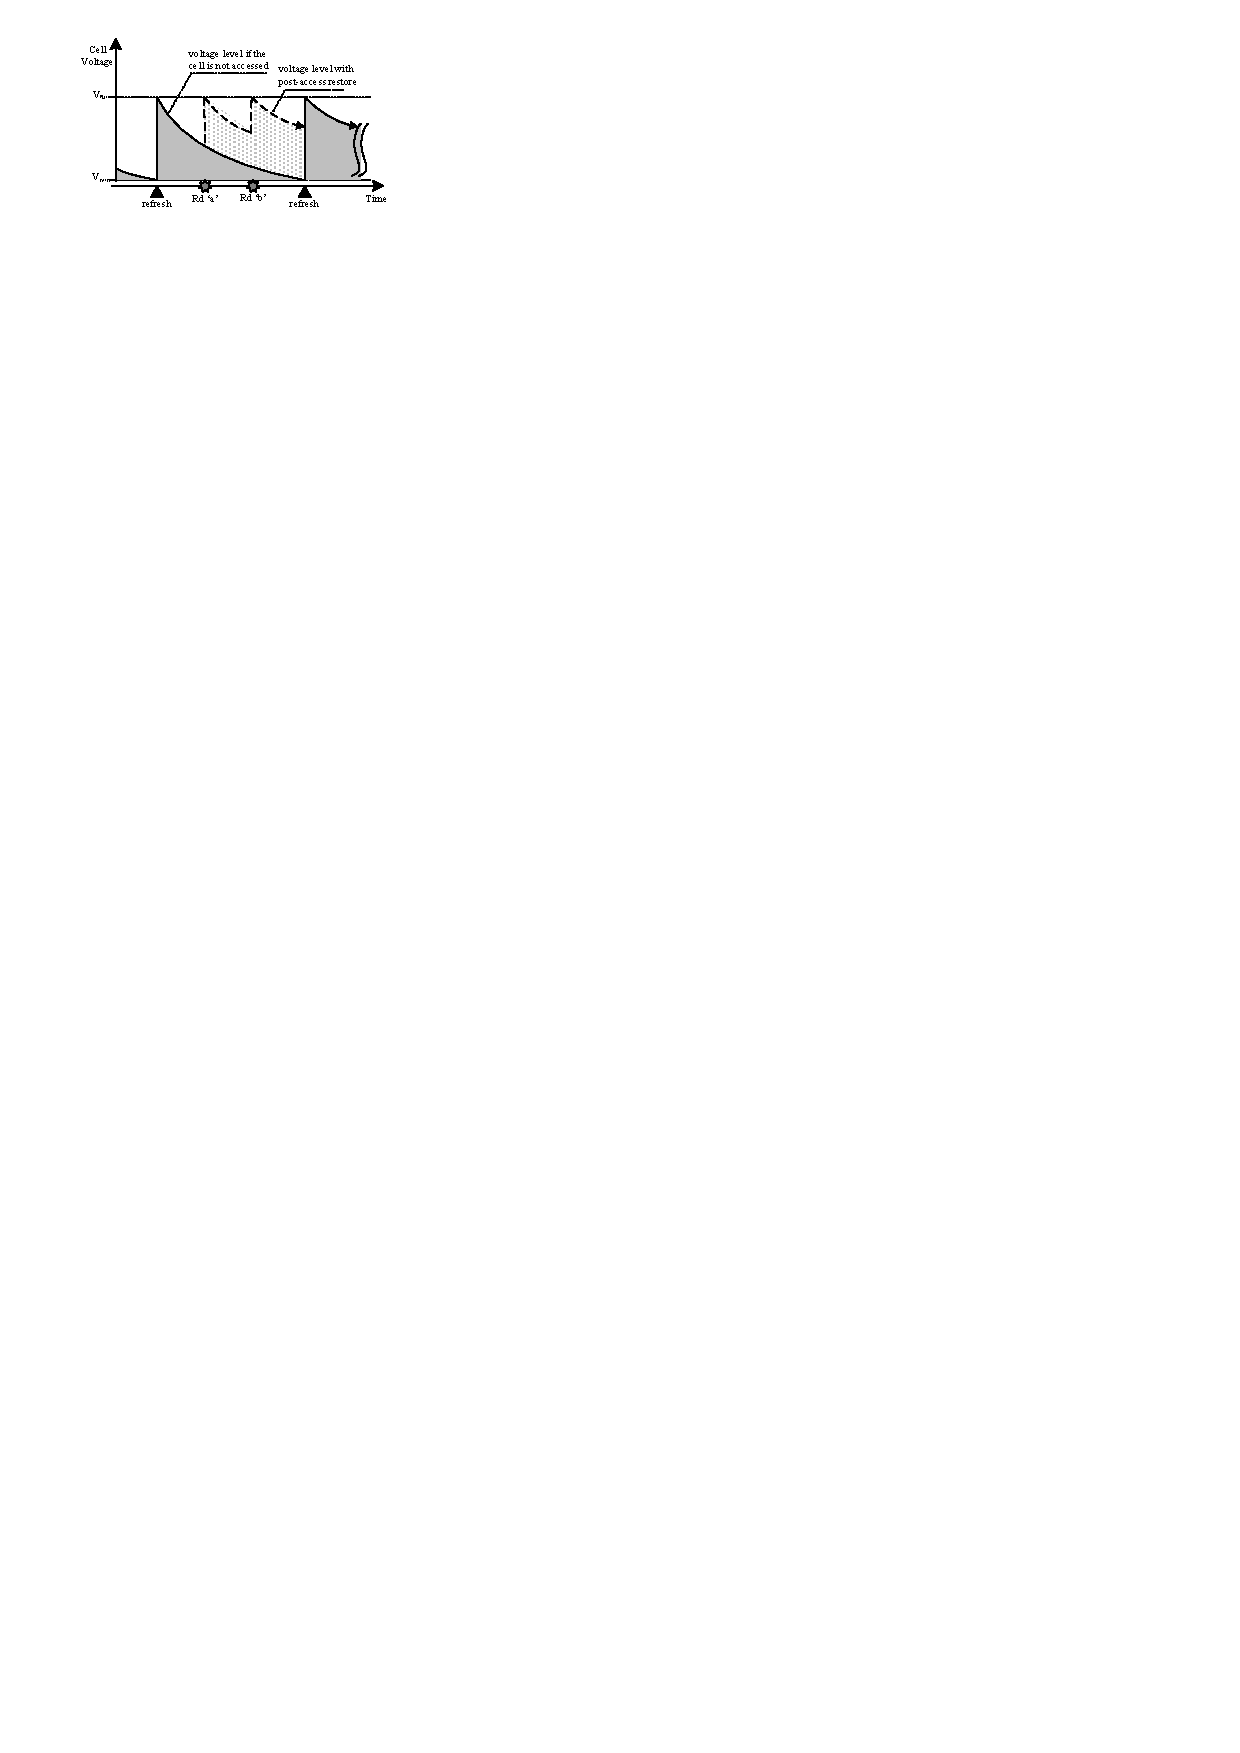
\includegraphics[width=3.2in]{figures/HPCA16/rt_partial.pdf}
\vspace{-0.2in}
\caption{DRAM cell voltage is fully restored by either refresh commands or memory accesses.  (V$_{full}$ indicates fully charged; V$_{min}$ is the minimal voltage to avoid data loss).}
\label{fig:partial}
\vspace{-0.3in}
\end{center}
\end{figure}

Based on this observation, we propose that post-access restore {\em partially charges} a cell's voltage to the level that the cell would have if the cell had been untouched in one refresh window. The restore operation is terminated when this target voltage level is reached. 

The cell charging curve starts with a deep slope and flattens when approaching V$_{full}$ \cite{HPCA15:aldram, PATENT11:dram}, as demonstrated in SPICE modeling. Hence, reducing target voltage can drastically shorten restore time. For example, SPICE modeling indicates that restoring a cell's charge to 0.89 V$_{dd}$ rather than 0.975 V$_{dd}$ (fully charged) reduces {\tt tWR} from 25 to 15 DRAM cycles, i.e., a 40\% reduction.

We next describe two schemes, {\tt RT-next} and {\tt RT-select}, to enable partial restore.  These schemes are applied by the memory controller.

\section{Proposed Designs}
\subsection{RT-next: Refresh-aware Truncation}

\begin{savenotes}
\begin{table*}[htbp]
\vspace{-0.2in}
\begin{center}
\caption{Adjusted restore timing values in {\tt RT-next}  (using the SPICE model)}
\vspace{-0.15in}
\label{rt_next_timing}
\scalebox{0.75}
{
\begin{tabular}{|c||c|c|c|c|*3c|}
\hline\hline
sub-window& \multicolumn{3}{|c|}{Distance to next refresh} & Target restore     &{\tt tRAS}	  &{\tt tWR}	  &{\tt tRCD}\\
            & 64ms-row & 128ms-row & 256 ms-row              & voltage (V$_{dd}$) &\multicolumn{3}{c|}{(DRAM cycles) \footnote{Timing values are gotten from SPICE modeling, more details can be found in \cite{HPCA16:twr}.}} \\ \hline \hline
1st         & [64ms, 48ms) & [128ms, 96ms) & [256ms, 192ms)  & 0.975		&42		&25	   	&15 \footnote{The studies focus on the relationship between restore and retention. Consequently, unrelated timing values, such as {\tt tRCD}, are unchanged.}  \\ \hline
2nd         & [48ms, 32ms) & [96ms, 64ms) & [192ms, 128ms)   & 0.92          	&27      &18    	&15  \\ \hline
3rd         & [32ms, 16ms) & [64ms, 32ms) & [128ms, 64ms)    & 0.86          	&21      &14    	&15  \\ \hline
4th         & [16ms, 0ms) & [32ms, 0ms) & [64ms, 0ms)        & 0.80          	&18      &11     &15  \\ \hline \hline
\multicolumn{4}{|c|}{No Truncation}            &0.975		&42		&25    	&15  \\ \hline \hline
%refresh margin &0.73          	&15      &9     &15  \\ \hline \hline
\end{tabular}
}
\end{center}
\vspace{-0.1in}
\end{table*}
\end{savenotes}

{\tt RT-next} truncates a long restore operation according to the time distance to its next refresh. %The sooner the next refresh is, the less charge the cells in the row need, and the earlier the restore operation can be terminated.  
%{\tt RT-next} works as follows. 
The refresh window is partitioned into multiple sub-windows, each of which provides a set of timing parameter values.
In the following, we use four sub-windows to discuss our proposed schemes --- Table \ref{rt_next_timing} lists the adjusted timing values for the device that we model in this paper. The smaller the timing values are, the larger opportunity the truncation has. While distinguishing more sub-windows provides finer-grained control and the potential to exploit more truncation benefits, it complicates the control and has diminishing benefits as shown in our experiments. 

As illustrated by Figure~\ref{fig:rtnext}, when servicing a read or write access, {\tt RT-next}  
calculates the time distance to the next refresh command and determine the sub-window that the access falls in. It then truncates its restore operation using the adjusted timing parameters, e.g., the right most columns in Table \ref{rt_next_timing}.

\begin{figure}[htbp]
\begin{center}
%\vspace{-0.1in}
\centering
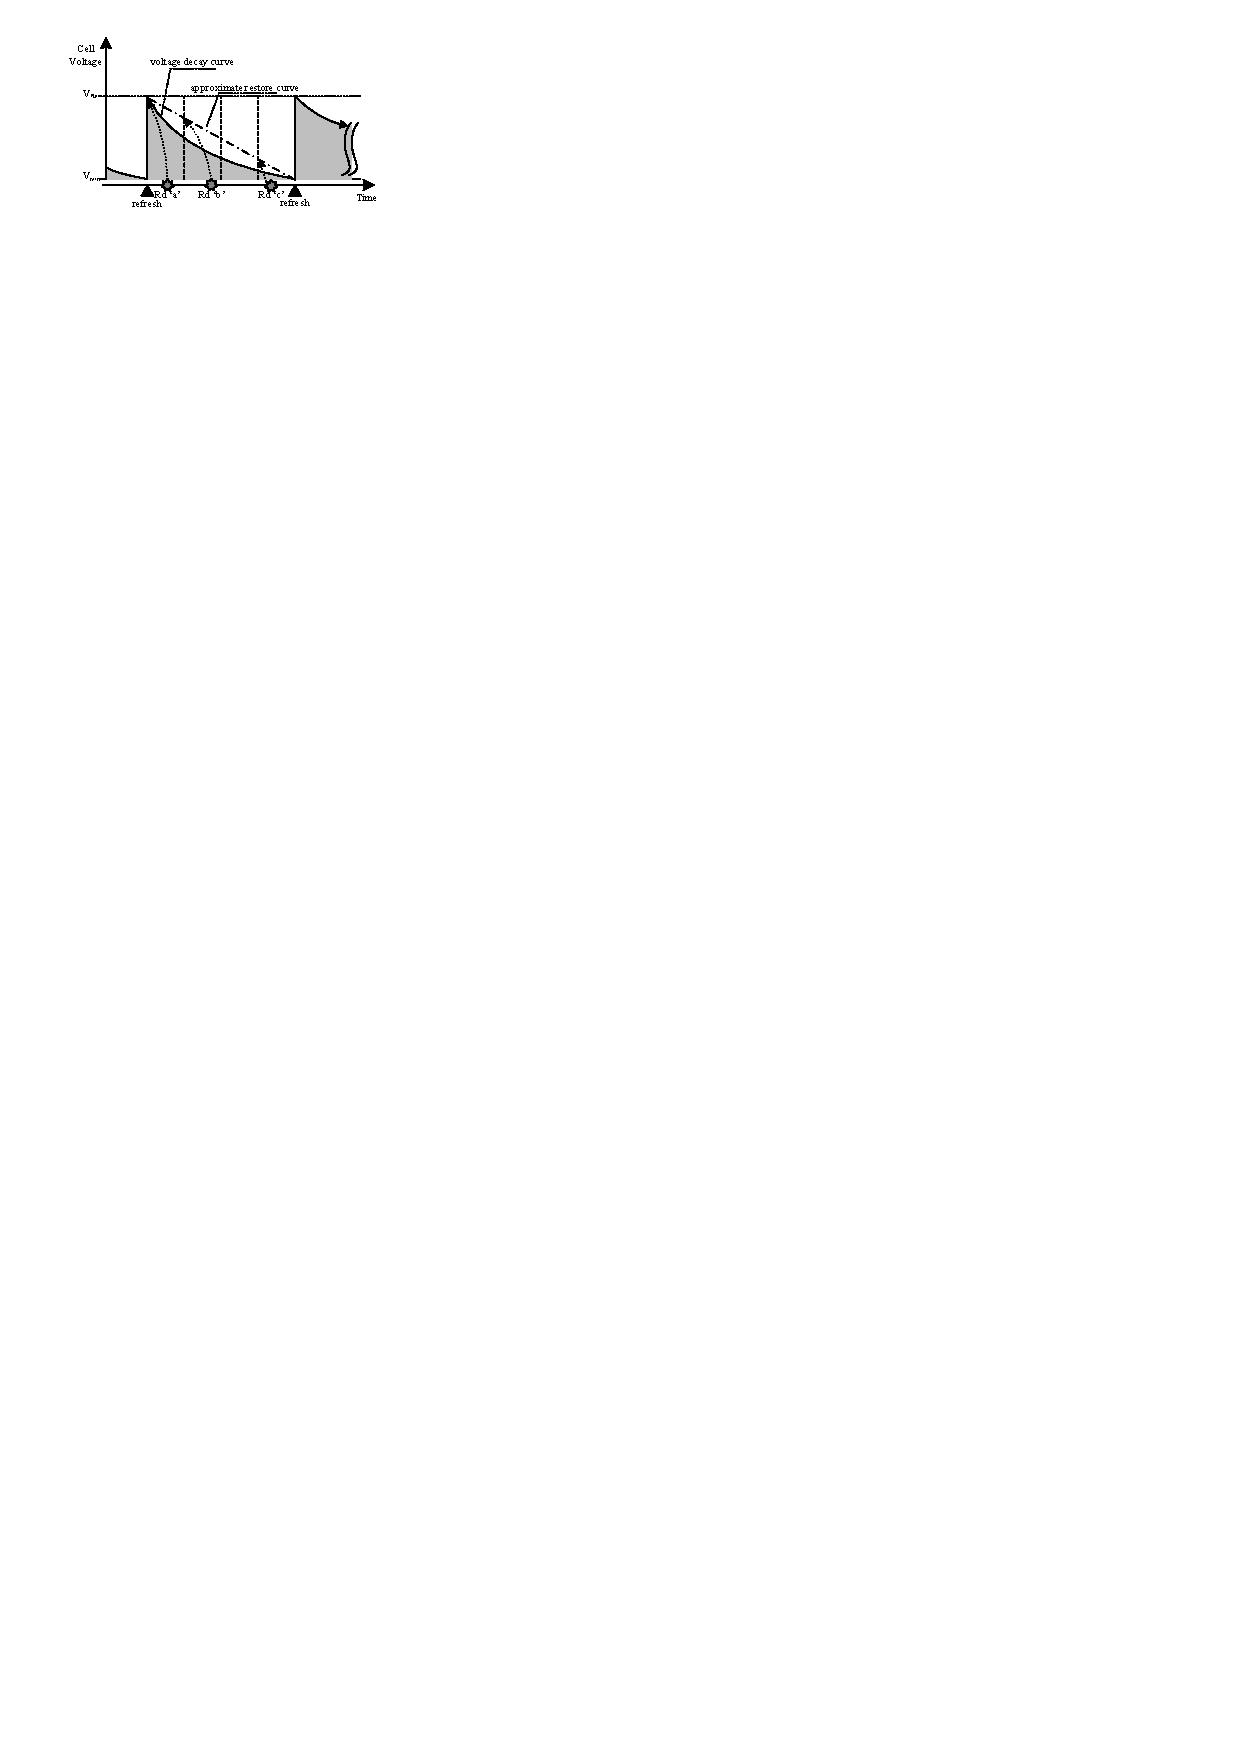
\includegraphics[width=3.2in]{figures/HPCA16/rt_next.pdf}
\vspace{-0.2in}
\caption{{\tt RT-next} safely truncates restore operation. Exponential curve has been verified from SPICE modeling, and linear line shows the conservative restoring goals.}
\label{fig:rtnext}
\vspace{-0.45in}
\end{center}
\end{figure}

%The memory controller also needs to consider the page policy (open or close).  A restore is truncated by a {\tt PRE} command from the memory controller. 
%For a close-page policy, every access can potentially truncate restore early. 
%For an open-page policy, truncating restore of a preceding access may not beneficial if its following access is a row buffer hit. 
%We evaluate both policies in the experiments.

%Figure~\ref{fig:rtnext} illustrates the working mechanism of {\tt RT-next}, where reads {\tt 'a'}, {\tt 'b'}, and {\tt 'c'} are serviced in the first, the second, and the fourth sub-windows, respectively.  Generally, {\tt RT-next} is a conservative approach to restore the cell charge.
%The figure shows how {\tt RT-next} is conservative in two ways:



%\footnotetext{\hi{Note that the negative slope is the conservatively approximated restore curve; the voltage decay curve, not shown in the figure, is always below the restore line.}}

%{\tt RT-next} is compatible with baseline auto refresh policy \cite{ISCA15:refresh, JEDEC:ddr3} that sends out {\tt REF} commands sequentially for all refresh bins. Given a DRAM row being accessed, the memory controller checks which bin the last {\tt REF} command is for and then determine how far the {\tt REF} is to be sent for the bin that the being accessed row resides.

\vspace{0.1in} 
{\underline{\bf {\tt RT-next} in multi-rate refresh.}}
\footnote{Retention time is modeled following \cite{EDL09:ret,ISCA12:raidr,ISCA13:archshield}, and leaky cells are randomly distributed based on prior works \cite{ISCA12:raidr, ISCA15:reflex, ICCD14:proactive}}
Applying {\tt RT-next} in a multi-rate refresh environment works similarly to the case that has only one rate. To calculate the distance between a memory access and the next refresh to its bin, 
{\tt RT-next} uses the same formula except adding the extra refresh rounds for low rate, i.e., 128/256ms, bins.
%replacing the refresh rate value with the individual refresh rate attached to each bin. 
Here we assume the underlying multi-rate refresh scheme has profiled and tagged each bin with its best refresh rate, e.g., 64ms, 128ms, or 256ms. 

As shown in Figure \ref{fig:rtnext_m}, it simplifies the timing control in memory controller by restoring a cell's post-access voltage according to the linear line between V$_{full}$ and V$_{min}$ (rather than the exponential decay curve). Given a 64ms-row and a 256ms-row, accesses falling in the same corresponding sub-window can use the same timing values in Table \ref{rt_next_timing}. 

\begin{figure}[htbp]
\begin{center}
\vspace{-0.1in}
\centering
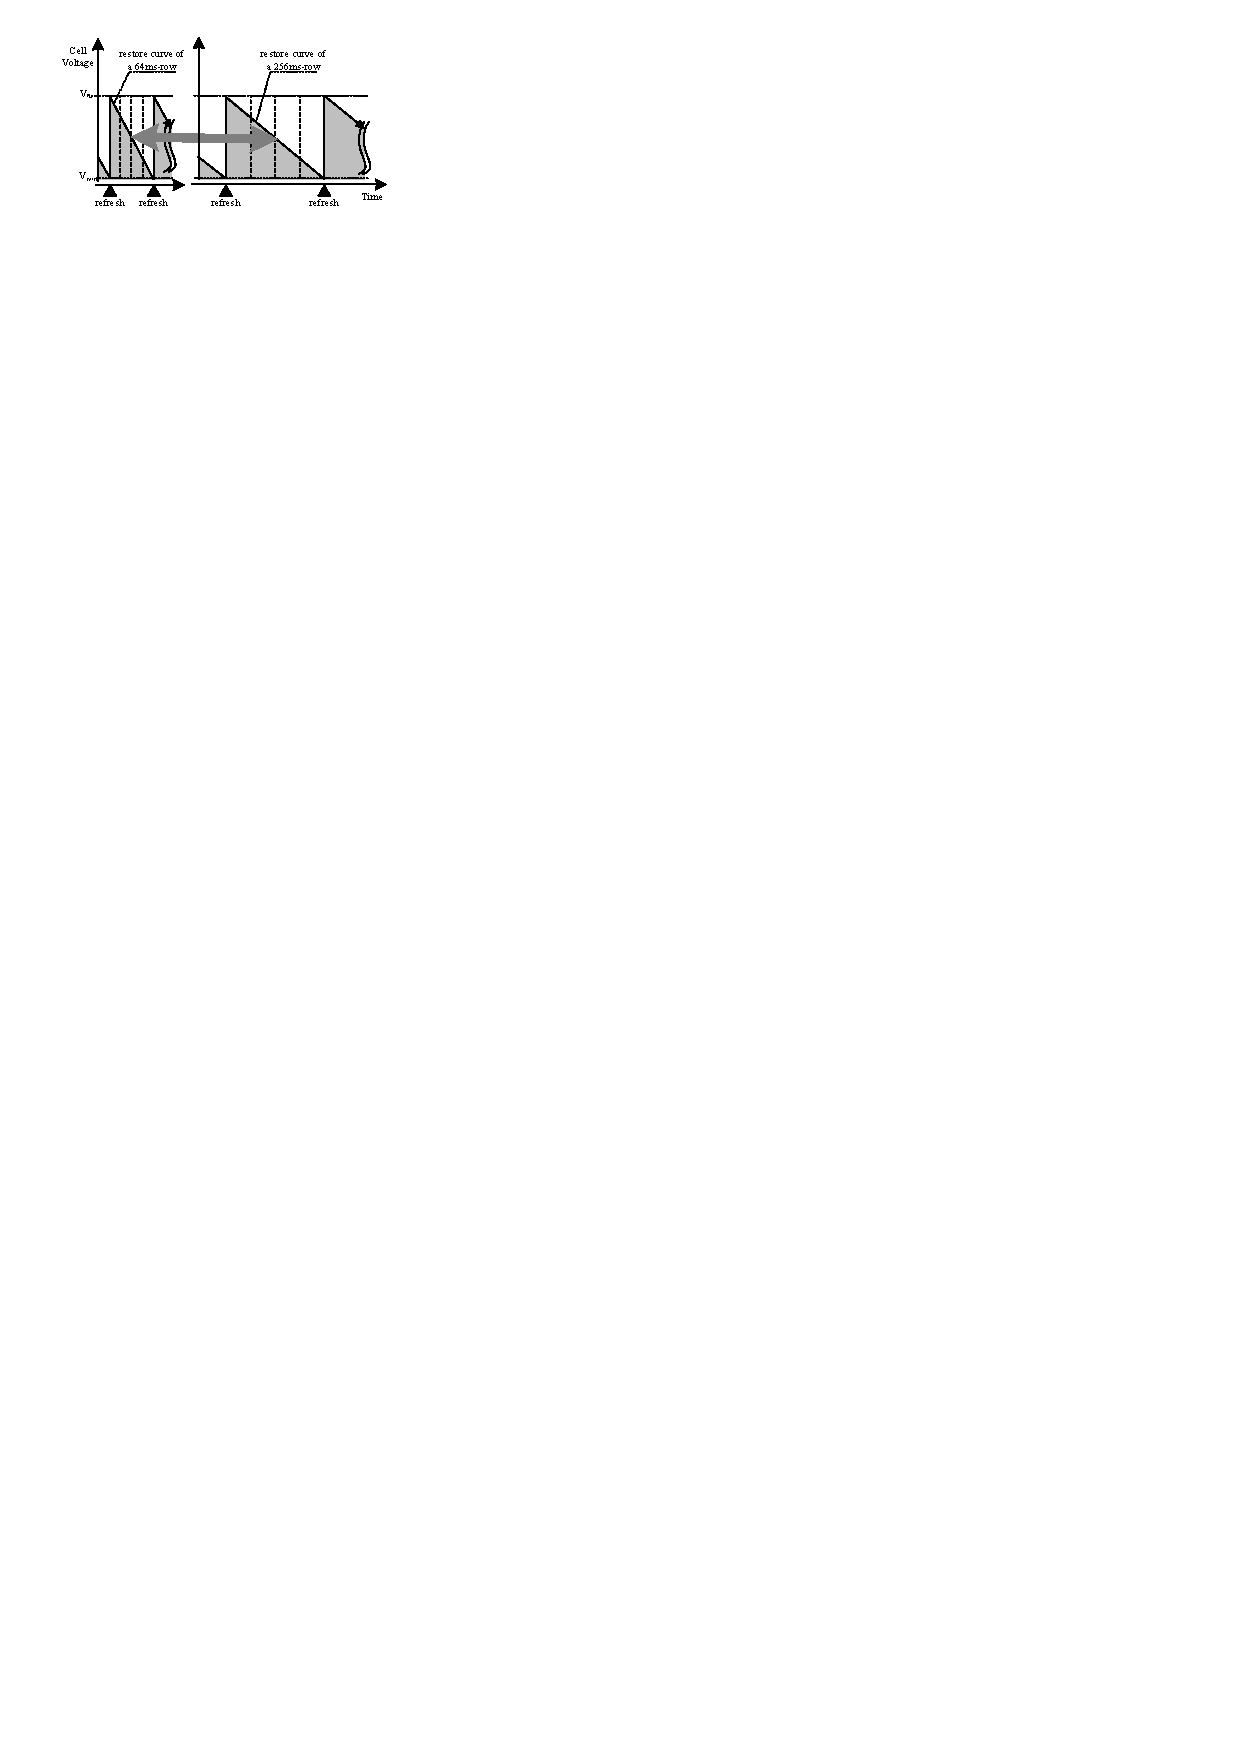
\includegraphics[width=3.2in]{figures/HPCA16/rt_next_m.pdf}
\vspace{-0.2in}
\caption{Restoring voltage according to linear line simplifies timing control in multi-rate refresh --- a 64ms-row and a 256ms-row share the same timing values in each correspond sub-window.}

\label{fig:rtnext_m}
\vspace{-0.45in}
\end{center}
\end{figure}

%In particular, although two different bins (e.g., 64ms and 256ms bins) have different sub-interval durations, they use the same adjusted timings (see Table \ref{rt_next_timing}). The same timings are used because, as shown in Figure \ref{fig:rtnext_m}, restore is conservatively performed using the approximated linear curve. 
%The cell loses about the same portion of charge within each sub-interval.
%The cell necessitates the same portion of charge within each sub-interval.
%\hi{Such interval division minimizes the required number of timing sets and thus greatly simply the design of memory controller}


\subsection{RT-select: Proactive Refresh Rate Upgrade}
Refresh and restore are two correlated operations that determine the charge in a cell. Less frequently refreshed bins can be exploited to further shorten the post-access restore time. 
We next present {\tt RT-select}, a scheme that upgrades refresh rate for more truncation opportunities. 

Figure \ref{fig:rtselective} illustrates the benefit of refreshing a 256ms-row (in multi-rate refresh) at 128ms rate.  Given that this row is a 256ms-row, its voltage level decreases to V$_{min}$ after 256ms. As shown in Figure \ref{fig:rtselective}(a), the refresh commands sent at +64ms, +128ms, and +192ms marks are dummy ones. The access ``Rd'' appears in the 2nd sub-window; it has a distance within [192ms, 128ms) to the next refresh command. According to {\tt RT-next}, the restore can be truncated after reaching 0.92V$_{dd}$ (using the 256ms-row column in Table \ref{rt_next_timing}).

Now, suppose the dummy refresh at +128ms is converted to a real refresh, i.e.,  the row is ``upgraded'' to a 128ms-row.  With this earlier refresh, 
%However, if the {\em dummy refresh at 128ms is converted to a real refresh (i.e., the 
%row is upgraded to a 128ms-row), then 
the access ''Rd'' is at most 64ms away from the next refresh. 
Using the 128ms-row column in the timing adjustment table, {\tt RT-next} 
can truncate the restore after it reaches 0.86V$_{dd}$, achieving significant timing 
reduction for the restore operation (Figure \ref{fig:rtselective}(b)).

%{\underline{if we convert the dummy refresh}}
%{\underline{command at 128ms mark to a real refresh, i.e., this row is}} \\
%{\underline{upgraded to a 128ms-row}}, access ``R$_a$'' is at most 64ms away from its next refresh. Using the 128ms-row column in the timing adjustment table, {\tt RT-next} can truncate the restore after it reaches 0.86V$_{dd}$, achieving significant timing reduction in restore operations.

\begin{figure*}[htbp]
\begin{center}
%\vspace{-0.1in}
\centering
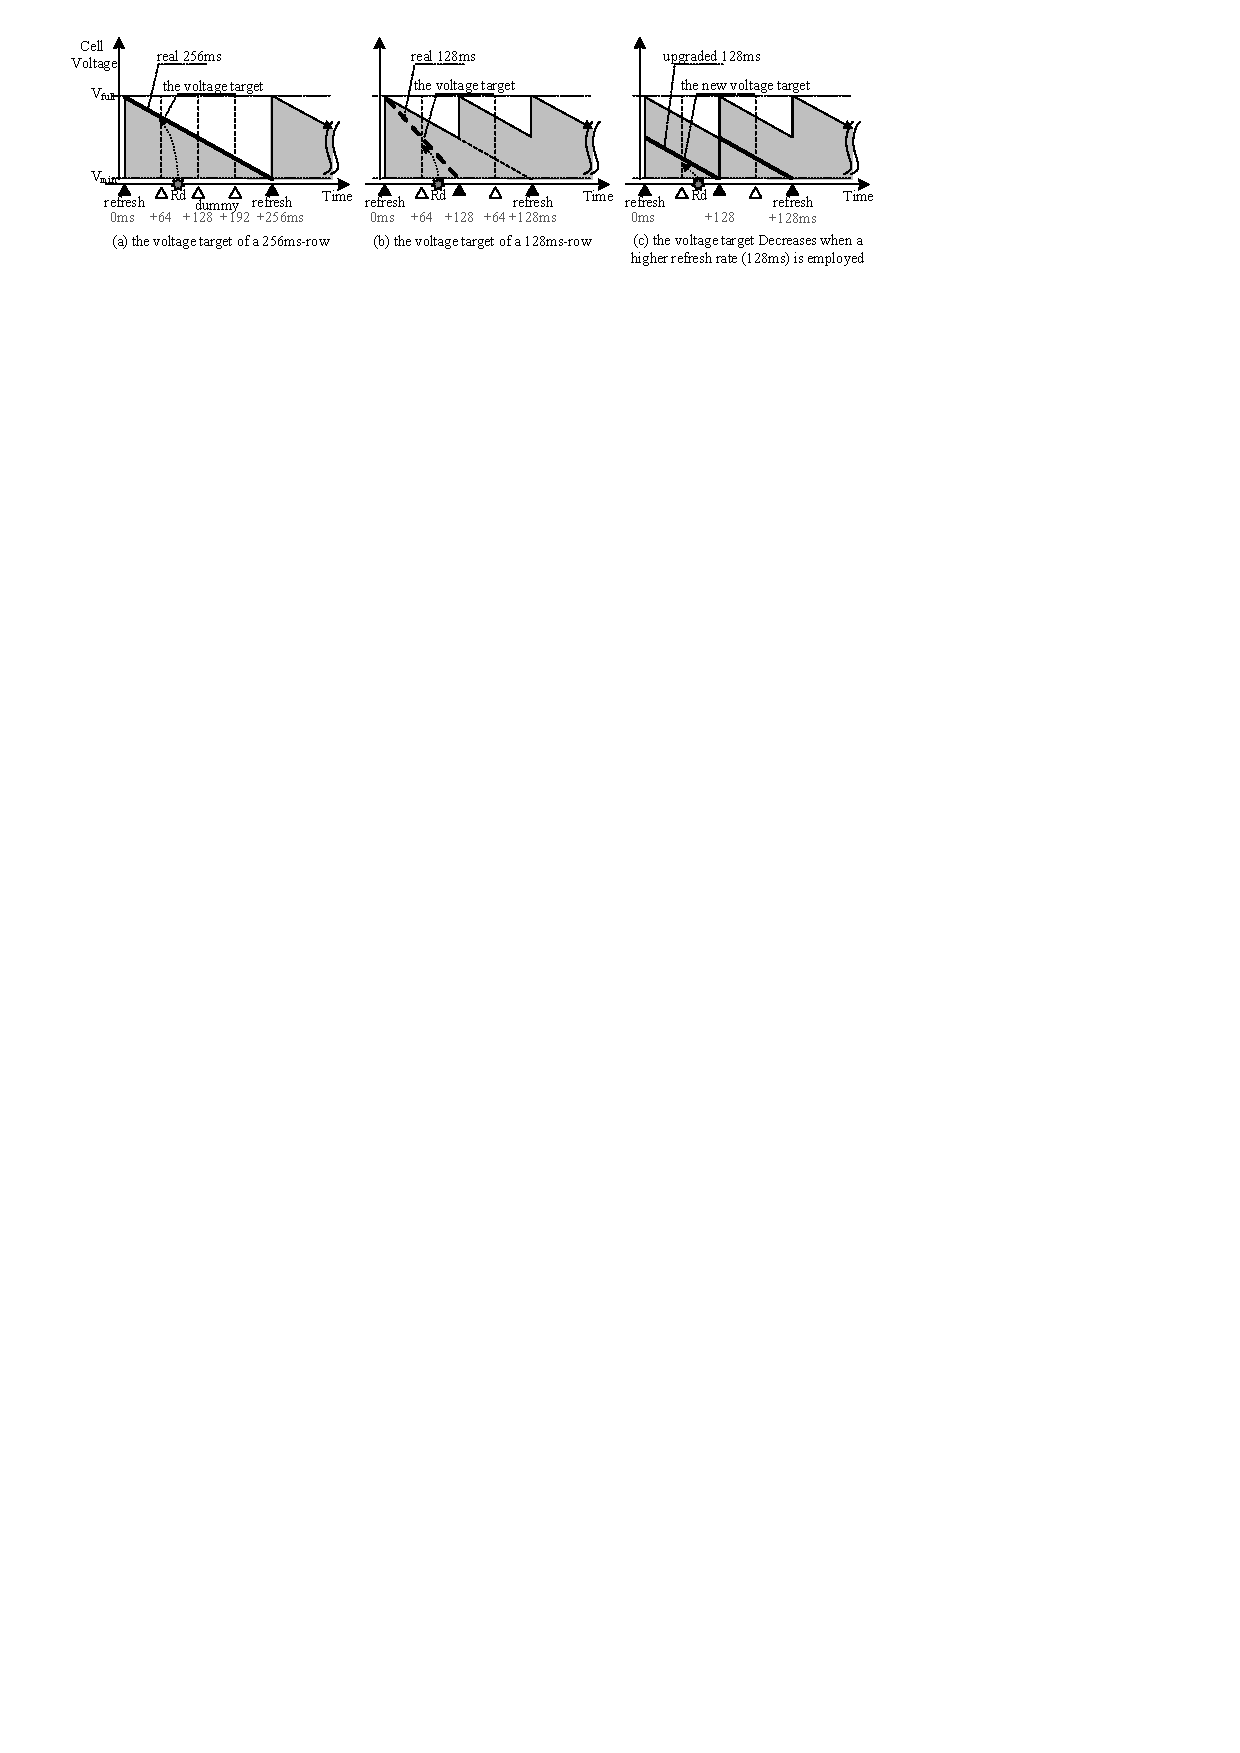
\includegraphics[width=6.4in]{figures/HPCA16/rt_selective.pdf}
\vspace{-0.2in}
\caption{The voltage target can be reduced if a strong row is refreshed at higher rate.}
\label{fig:rtselective}
\vspace{-0.3in}
\end{center}
\end{figure*}

Refreshing a 256ms-row at 128ms rate exposes more truncation benefits, as shown in 
Figure \ref{fig:rtselective}(c). For access "Rd'', it is sufficient to restore the voltage to 0.80V$_{dd}$ rather than 0.86V$_{dd}$ in above discussion. 
This is because a 256ms-row, even if being refreshed at 128ms rate, leaks slower than a real 128ms-row. We can adjust the timing values by following the solid thick line in \ref{fig:rtselective}(c), rather than the dashed thick line from a real 128ms-row, as shown in \ref{fig:rtselective}(b).
In particular, %as summarized in Table \ref{rt_selective_timing}, 
a row access, even if it is 128ms away from the next refresh to the row, just needs to restore the row to 0.86V$_{dd}$, rather than V$_{full}$ (=0.975V$_{dd}$) for a real 128ms-row. 

%\begin{table}[htbp]
%\vspace{-0.2in}
%\begin{center}
%\caption{Adjusted restore timing values in {\tt RT-select}}
%\vspace{-0.2in}
%\label{rt_selective_timing}
%\scalebox{0.7}
%{
%\begin{tabular}{|c||c|c|*3c|}
%\hline\hline
%Upgrade       &  Distance to Next  & Target restore      &{\tt tRAS}	  &{\tt tWR}	  &{\tt tRCD}\\
%              &  refresh           &  voltage (V$_{dd}$) &\multicolumn{3}{c|}{(DRAM cycles)} \\ \hline \hline
%256ms-$>$128ms  & [128ms, 64ms)      & 0.86 		&21		   &14	   	&15  \\ \cline{2-6}
%              & [64ms, 0ms)        & 0.80     &18      &11    	&15  \\ \hline \hline
%256ms-$>$64ms   & [64ms, 0ms)        & 0.80 		&18		   &11	   	&15  \\ \hline \hline
%128ms-$>$64ms   & [64ms, 32ms)        & 0.86 		&21		   &14	   	&15  \\ \cline{2-6} 
%			 & [32ms, 0ms)        & 0.80 		&18		   &11	   	&15  \\ \hline \hline 
%\end{tabular}
%}
%\end{center}
%\vspace{-0.1in}
%\end{table}

{\bf RT-select scheme.} 
While upgrading refresh rate reduces restore time, it generates more real refresh commands, which not only prolongs memory unavailable period but also consumes more refresh energy. 
Previous work shows that refresh may consume over 20\% of the total memory energy for a 32Gb DRAM device \cite{TC15:refresh, ISCA12:raidr}. Blindly upgrading the refresh rate of all rows is thus not desirable.

{\tt RT-select} upgrades the refresh rate of {\em selected bins}, those were touched, for {\em one refresh window}. It works as follows. 
A 3-bit rate flag is attached to each refresh bin to support multi-rate refresh. 
When there is a need to upgrade, e.g., from 256ms to 128ms rate, {\tt RT-select} updates the rate flag as shown in section~3.5, which converts the dummy refresh at +128ms in Figure~\ref{fig:rtselective}. 
A real refresh command rolls the rate back to its original rate, i.e., {\tt RT-select} only upgrades the touched bin for one refresh window, which incurs modest refreshing overhead to the system.

\section{Architectural Enhancements}

To enable {\tt RT-next} and {\tt RT-select}, we enhance the memory controller, as shown in Figure~\ref{fig:arch}. RT adds a truncation controller, to adjust the timing for read, write, and refresh accesses. This control is similar to past schemes that change timings \cite{HPCA13:tldram, ISCA13:charm, HPCA14:nuat}.  The memory controller has a register that records the next bin to be refreshed, referred to as {\tt Bin$_c$}, which rolls over every 64ms. 
It can also infer the mapping from row address to refresh bin, the same as that in \cite{ISCA15:reflex, ISCA14:disturbance}. 

To support multi-rate refresh, the memory controller keeps a small table that uses 3 bits to record the refresh rate of each refresh bin, similar to that in \cite{ISCA12:raidr, ISCA15:reflex}. As shown in Table \ref{tab:flag}, a 64ms-/128ms-/256ms- bin is set as `000'/`01A'/`1BC', respectively. Here `A' and `BC' are initialized to ones and decrement every 64ms.
While the refresh bin counter increments every in 7.8$\mu$s(=64ms/8192), a real {\tt REF} command is sent to refresh the corresponding bin only if its bin flag is `000', `010', or `100'. 
`A' and `BC' are changed back to `1' and `11' afterwards, respectively.

\begin{figure}[htbp]
\begin{center}
%\vspace{-0.1in}
\centering
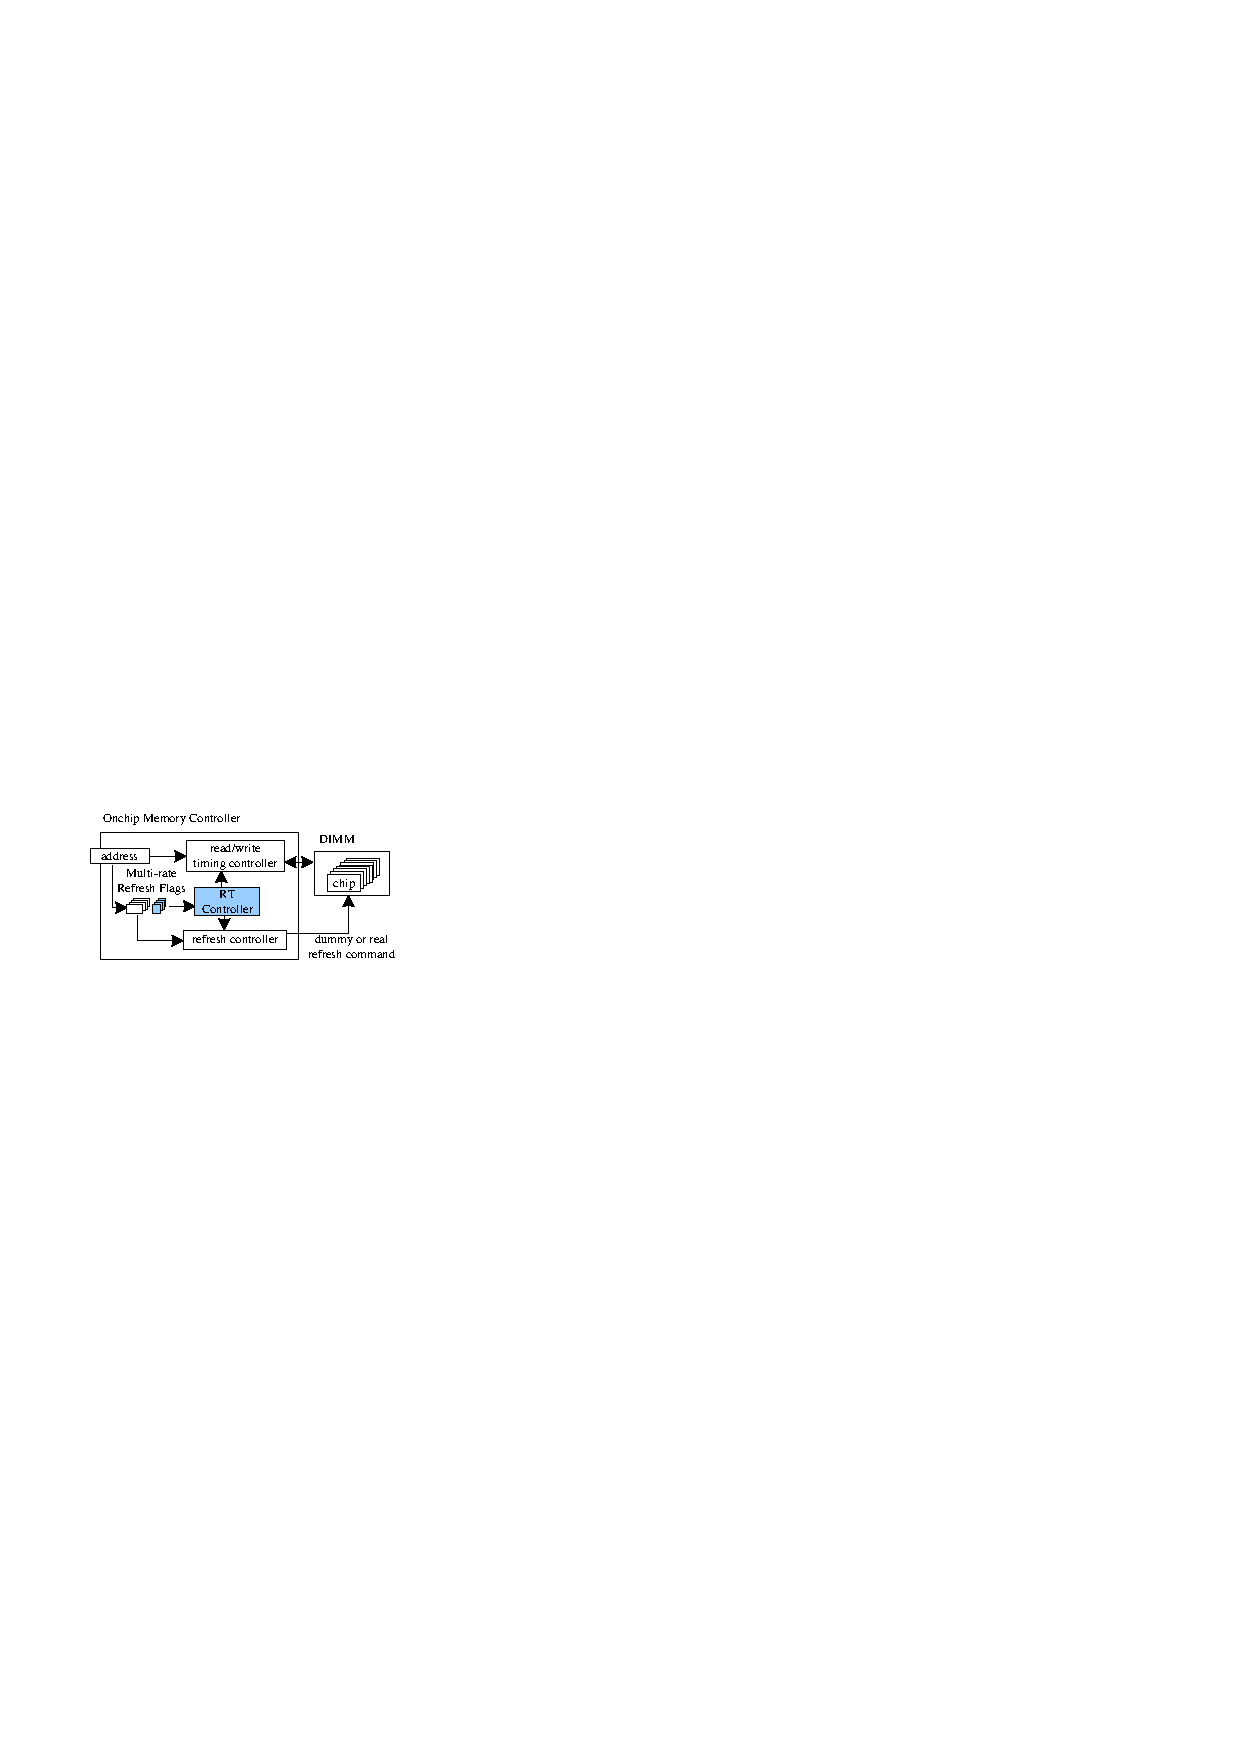
\includegraphics[width=3.25in]{figures/HPCA16/rt_arch.pdf}
\vspace{-0.1in}
\caption{The RT architecture (the shaded boxes are added components).}
\label{fig:arch}
\vspace{-0.45in}
\end{center}
\end{figure}

When upgrading the refresh rate of a refresh bin, we update the rate flag according to the last column in Table \ref{tab:flag}. For example, when upgrading a 128ms-bin to 64ms rate, we set the rate flag as `010', which triggers the refresh in the next 64ms duration and roll back to `011' afterwards. This effectively upgrades for one round. Upgrading 256ms-row to 128ms rate sets the flag as `1BC$\oplus$0B0', which always sets the middle bit to zero to ensure that the refresh distance is never beyond 128ms, and thus the sub-window can only be {\tt 3rd} and {\tt 4th} referring to Table \ref{rt_next_timing}. In general, the distance calculation in {\tt RT-select} is adjusted by adding further refresh rounds indicated by the two least significant bits (LSB) of rate flag.

 \begin{table}[htbp]
 \vspace{-0.25in}
\caption{Refresh rate adjustment table}
\vspace{-0.3in}
\begin{center}
\scalebox{0.8}
{
\begin{tabular}{l|l|l}
\hline \hline 
{Profiled refresh rate}	&{Rate flag}	&{Flag after rate upgrade}\\
\hline\hline
64ms		&$000$	& n/a\\
\hline
128ms		&$01A$	&128$\rightarrow$64ms: 010\\
\hline
256ms		&$1BC$	&256$\rightarrow$128ms: 1BC$\oplus$0B0\\
			&		&256$\rightarrow$64ms: 100\\
\hline\hline
\end{tabular}
}
\end{center}
\label{tab:flag}
%\vspace{-0.2in}
\end{table}

To enable multi-rate refresh, the %3KB (=3bits*8192) 
rate table is accessed before each refresh to determine if a real or dummy command should be sent. To enable {\tt RT-select}, the rate table is also 
accessed before each memory access to decide the refresh distance, and then to complete the upgrade after the access.
%accessed before each memory access to decide if it is necessary to upgrade the rate. 
The extra energy is minimal, as shown in Section~\ref{subsec:energy}.

\section{Experimental Methodology}\label{sec:experiment}
\subsection{Configuration}\label{subsec:setting}
To evaluate the effectiveness of our proposed designs, we performed the simulation using the memory system simulator USIMM \cite{SIMU:usimm}, which simulates DRAM system with detailed timing constraints. 
USIMM was modified to conduct a detailed study of refresh and restore operations.

We simulated a quad-core system with settings listed in Table \ref{tab:configuration}, similar to those in \cite{HPCA13:refresh_pausing, HPCA14:nuat}. 
The DRAM timing constraints follow Micron DDR3 SDRAM data sheet \cite{SIMU:datasheet}. By default, DRAM devices are refreshed with 8K {\tt REF} within 64ms, and {\tt tRFC} is 208 DRAM cycles, which translates into a {\tt tREFI} of 7.8 $\mu$s (i.e., 6240 DRAM cycles). As  \cite{HPCA13:refresh_pausing}, the baseline adopts closed page policy, which works better in multicore systems \cite{PACT12:close_page}. 

\begin{table}[htbp]
\vspace{-0.2in}
\caption{System Configuration}
\vspace{-0.3in}
\begin{center}
\scalebox{0.8}
{
\begin{tabular}{l|l}
\hline\hline
Processor			&four 3.2Ghz cores; 128 ROB size\\
				&Fetch width: 4, Retire width: 2, Pipeline depth: 10\\
\hline
				&Bus frequency: 800 MHz\\
 				&Write queue capacity: 64\\
Memory			&Write queue watermarks: 40/20\\	
Controller			&Address mapping: rw:cl:rk:bk:ch:offset\\
				&Page management policy: close-page with FRFCFS\\

\hline
				&2channels, 1rank/channel, 8banks/rank, \\
DRAM			&64K rows/bank, 8KB/row, 64B cache line\\
				&tCK=1.25ns, width: x8\\
%DRAM			%&tCAS(CL): 13.75ns, tRCD: 13.75ns, tRC: 48.75ns\\
				%&tCWD: 6.25ns (5 cycles), tBURST: 5.0ns (4 cycles)\\
				%&tRAS: 35ns, tRP: 13.75ns, tFAW: 24 cycles,\\
				%&tRRD: 5 cycles, tRFC: 208nCK, tREFI: 7.8$\mu$s\\
\hline\hline

\end{tabular}
}
\end{center}
\label{tab:configuration}
\vspace{-0.4in}
\end{table}

\subsection{Workloads}
For evaluation, we use workloads from the Memory Scheduling Championship \cite{SIMU:msc}, which covers a wide variety of benchmarks, including five commercial applications \textit{comm1} to \textit{comm5}, nine benchmarks from PARSEC suite and two benchmarks each from the SPEC suite and the Biobench suite. Among them, \textit{MT-fluid} and \textit{MT-canneal} are two multithreaded workloads.
As \cite{HPCA13:refresh_pausing}, the benchmarks are executed in rate mode, and the time to finish the last benchmark is computed as the execution time.


\section{Results}\label{sec:results}

%\subsection{Schemes to Study}
We evaluated our proposed RT schemes on system performance, memory access latency and energy, and then studied their sensitivities to different configurations.
To study different aspects of RT, we analyze different set of schemes in each figure.

\subsection{Impact on Performance}

Figure \ref{fig:time} compares the execution time of different schemes.
The results are normalized to \texttt{Baseline}. 
In the figure, {\tt Gmean} is the geometric mean of the results of all workloads.

\begin{figure*}[htbp] 
\centering
\centering
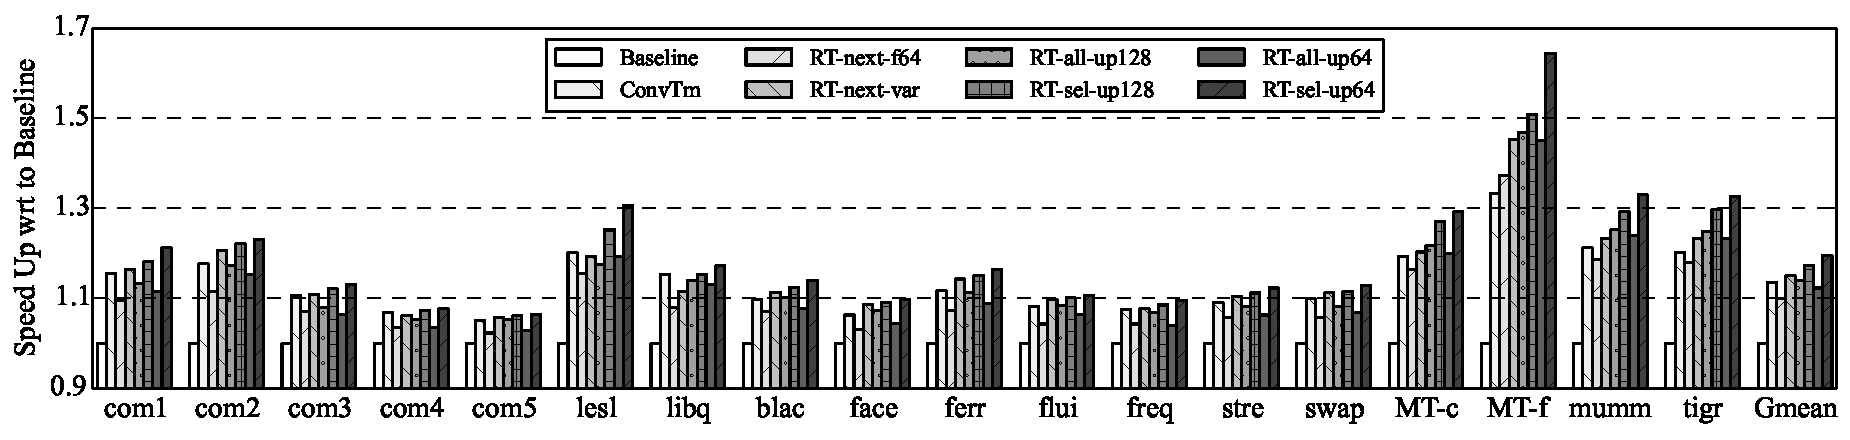
\includegraphics[width=6.5in]{{figures/HPCA16/DATA/0903.dat/4Gb/stat_4Gb_Cycles.perc.main.dat}.pdf}
\vspace{-0.45in}
\caption{Performance comparison of different schemes. {\tt Baseline} and {\tt ConvTm} adopts projected and conventional timings, respectively; {\tt NoRefresh} assumes no refresh activity in {\tt Baseline}; {\tt RT-next-XX} truncates restore based on its distance to next fresh, and {\tt f64} and {\tt var} supports fixed 64ms refresh rate and multiple rates, respectively; {\tt RT-all-upYY} aggressively upgrades refresh bins with rates lower than {\tt YY} to {\tt YY}; finally, {\tt RT-sel-upYY} are optimized schemes to balance the restore benefits and refresh overhead.}
\label{fig:time}
\vspace{-0.45in}
\end{figure*}

On average, \texttt{RT-next-f64} achieves 10\% improvement over {\tt Baseline} by truncating restore time. {\tt RT-next-var} identifies more truncation opportunities in multi-rate refresh DRAM modules and achieves better, i.e., 15\%, improvement. 
While {\tt RT-all-up128} truncates more restore time through refresh rate upgrade, it introduces extra refresh overhead and thus is slightly worse than {\tt RT-next-var}.
\texttt{RT-sel-up128} achieves 2.4\% improvement over \texttt{RT-next-var}
by balancing refresh operations and restore benefits. 
The performance gap between upgrading all rows and selective upgrading is even larger when we aggressively upgrade refresh rate to 64ms. \texttt{RT-sel-up64} achieves the best performance --- it is 19.5\% speedup over {\tt Baseline}, or 4.5\% better than \texttt{RT-next-var}.
The performance trend across the schemes demonstrates that our restoring schemes achieves a good balance between refresh and restore.

%Generally, memory access intensive workloads such as \textit{com1}, \textit{libq} and \textit{mumm} benefit most from the reduced restore timing.
%Particularly, \textit{MT-f} obtains the largest performance improvement because of the parallel access patterns and relatively tight gaps between accesses, which greatly enlarges the effect of shortened {\tt RAS} and {\tt WR}.

\subsection{Energy Consumption}\label{subsec:energy}
Figure \ref{fig:energy} compares the energy consumption of different schemes. 
We reported the energy consumption breakdown ---  background ({\tt bg}), activate/precharge ({\tt act/pre}), read/write ({\tt rd/wr}) and refresh ({\tt ref}). We summarized the results according to benchmark suites, where results are averaged over workloads within each suite.
We used the Micron power equations \cite{TOOL:power}, and the parameters from vendor data sheets \cite{SIMU:datasheet} with scaling. 

To enable truncation in multi-rate refresh DRAM modules, we need to query the refresh rate for each access. The refresh rates for 8192 bins are organized as 3KB direct mapped cache with 8B line size. We used CACTI5.3 \cite{URL:cacti} to model the cache with 32nm technology --- it requires 0.22ns access time, occupies 0.02mm$^2$ area, consumes 1.47mW standby leakage power, and spends 3.33pJ energy per access. The extra energy is trivial (less than 0.5\%) and is reported together with {\tt bg}. 

\begin{figure}[htbp] 
%\vspace{-0.1in}
\begin{center}
\centering
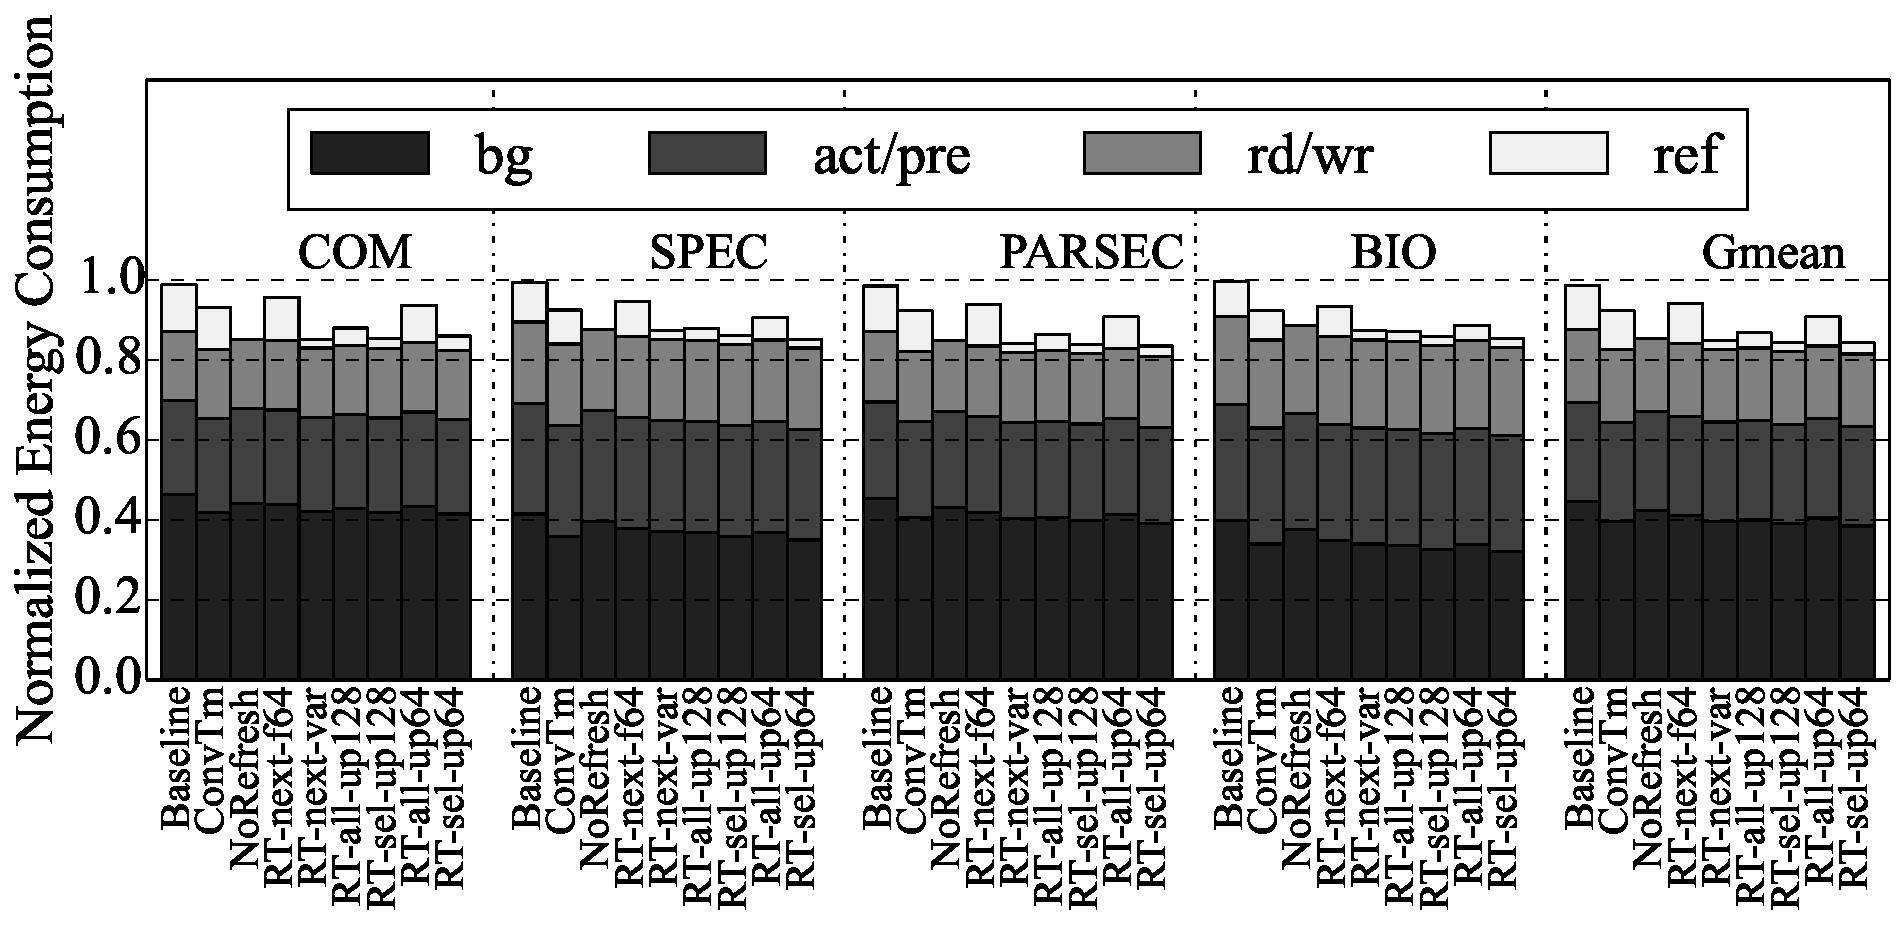
\includegraphics[width=0.7\textwidth]{{figures/HPCA16/DATA/0903.dat/4Gb/stat_4Gb_energy.all.dat.cat}.pdf}
\vspace{-0.1in}
\caption{Comparison of memory system energy.}
\label{fig:energy}
\end{center}
\vspace{-0.4in}
\end{figure}

From the figure, we observed that the device refresh energy for 4Gb chips is small. 
Due to increased refresh operations, {\tt RT-all-up128/-up64} consume much more refresh energy than {\tt RT-all-up128/-up64}, respectively. \texttt{RT-sel-up64} saves 17\% energy compared to {\tt Baseline}, and consumes slightly lower energy than \texttt{NoRerefresh} due to decreased execution time. And, as expected, {\tt RT-sel-} refresh schemes is more energy efficient than {\tt RT-all-} refresh peers.


\subsection{Comparison against the State-of-the-art}
Figure \ref{fig:state} compares RT with three related schemes in the literature. 
\begin{itemize}
\itemsep -1pt
\item
{\tt Archshield+} implements a scheme that treats all the cells with long restore latency as failures and adopts Archshield \cite{ISCA13:archshield} to rescue them. 
\item
{\tt MCR} is the recently proposed scheme that trade DRAM capacity for better timing parameters \cite{ISCA15:mcr}. {\tt $2x$ MCR} and {\tt $4x$ MCR} are the two options that reduce DRAM capacity to 50\% and 25\% of the original, respectively.
\item
{\tt ChunkRemap} implements the scheme that differentiates chunk level restore difference and constructs fast logic chunks through chunk remapping \cite{DATE15:twr}. 

\end{itemize}

\begin{figure}[htbp] 
\begin{center}
\centering
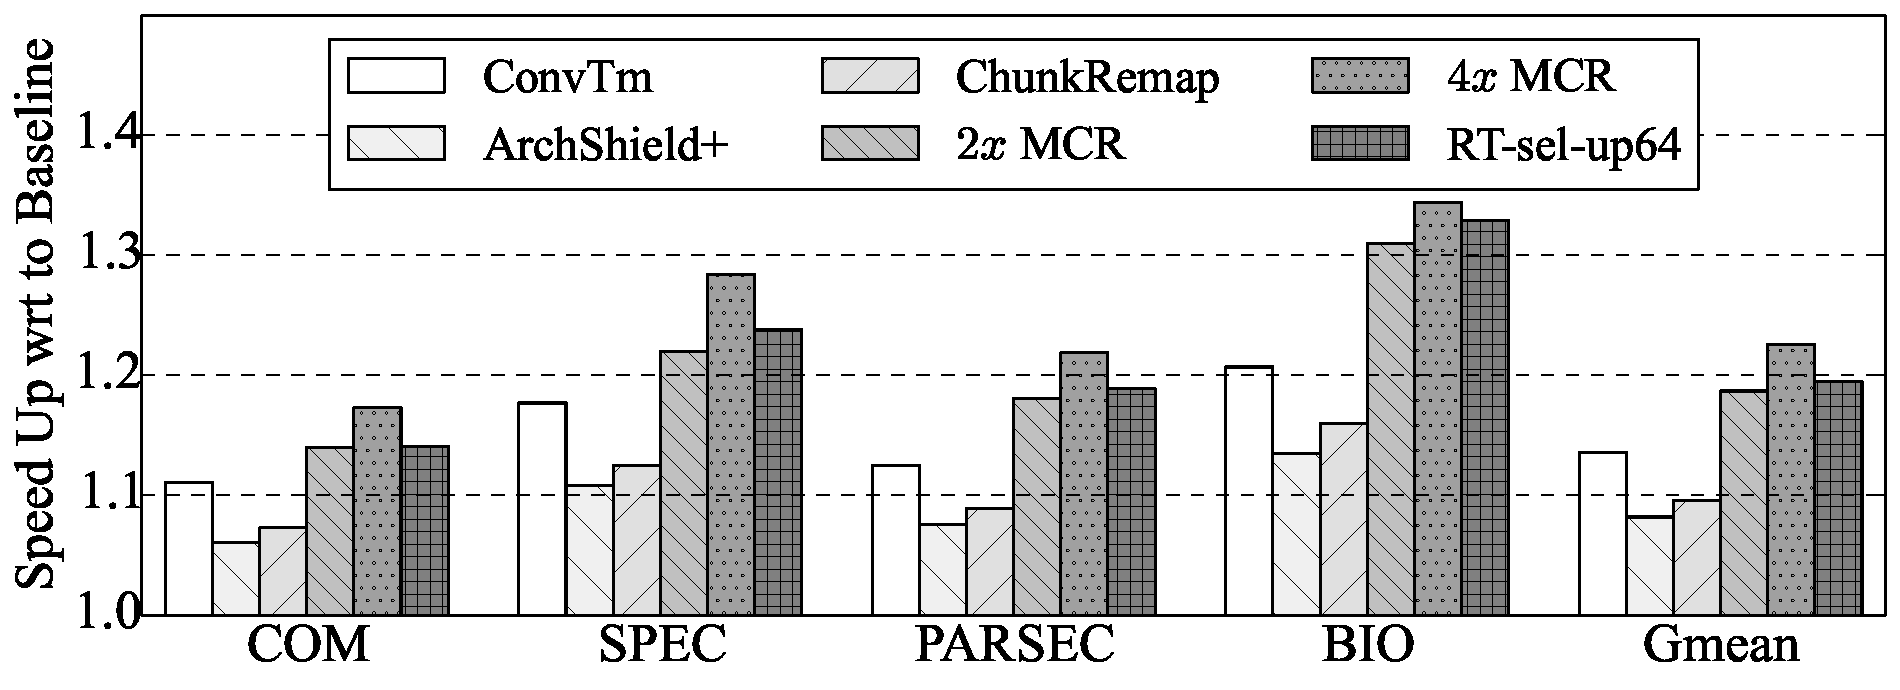
\includegraphics[width=3.4in]{{figures/HPCA16/DATA/0903.dat/4Gb/stat_4Gb_Cycles.perc.statart.dat}.pdf}
\vspace{-0.2in}
\caption{Comparison against the state-of-the-art.}
\label{fig:state}
\vspace{-0.45in}
\end{center}
\end{figure}

The figure shows that {\tt Archshield+} and {\tt ChunkRemap} are approaching {\tt ConvTm} while {\tt RT-sel-up64} is 5.2\% better than {\tt ConvTm}, exploiting more benefits from reduced restore time.
{\tt $4x$ MCR} outperforms {\tt RT-sel-up64} by a modest percentage, and {\tt RT-sel-up64} works better than {\tt $2x$ MCR}.

{\tt MCR} shares similarity with {\tt RT-select}, i.e., we share the observation that a line that is refreshed more frequently can be restored to a storage level lower than V$_{full}$. {\tt MCR} exploits this with significant DRAM capacity reduction while {\tt RT-select} takes a light weight design that upgrades used bins only for one refresh window, and leaves all the other bins being refreshed at original rates. 

%From the figure, {\tt $4x$ MCR} outperforms {\tt RT-sel-up64} by a modest percentage. 
%This is because {\tt MCR} improves the baseline by reducing not only restore time but also sensing time while {\tt RT-sel-up64} focuses only restore time. 
%{\tt RT-sel-up64} works better than {\tt $2x$ MCR} because it upgrades the refresh rate of a bin for one refresh window at a time, which significantly reduces refresh overhead (as shown with the difference from {\tt RT-all-up64}). 



%By focusing on restoring and respecting the DRAM auto-refresh, we only improve tRAS and tWR in this paper, whereas {\t MCR} reduces both tRCD and tRFC besides tRAS \footnote{Although {\tt MCR} \cite{ISCA15:mcr} failed to take write restoring (tWR) into account in the paper, for a fair comparison, we embed tWR reductions into MCR schemes.}
%. 
%Nevertheless, the figure shows that our proposed {\tt RT-sel-up64} outperforms {\tt MCR-2} and approaches {\tt MCR-4} (the gap is within 3\%).
%The performance difference is pretty narrow because: (1) our RT schemes take use of the multi-rate refresh to do restoring, which is capable to achieve restoring reduction and refresh improvement simultaneously comparing to {\tt Baseline}; to the contrary, {\tt MCR} ignored the retention time variation to use a fixed 64ms refresh rate; (2) RT schemes combines distance-aware restore and refresh rate upgrade, which makes the best timing values outperform those can be achieved by {\tt MCR}.


\begin{table}[htbp]
\vspace{-0.2in}
\caption{Comparing EDP between RT and MCR (lower is better).}
\vspace{-0.3in}
\begin{center}
\scalebox{0.8}
{
\begin{tabular}{*5c}
\hline\hline
Cases		& {\tt ConvTm} & {\tt RT-sel-up64}	& {\tt $2x$ MCR}	&{\tt$4x$ MCR-4}\\
\hline
\texttt{Same Chip}	& 1.0$\times$ &0.715$\times$		&0.753$\times$		&0.713$\times$\\
\texttt{Same Capacity}	& 1.0$\times$  &0.715$\times$		&0.918$\times$		&1.068$\times$\\
\hline\hline

\end{tabular}
}
\end{center}
\label{tab:edp}
\vspace{-0.45in}
\end{table}

Given that {\tt MCR} improves performance at a significant capacity reduction.
We next comparing the energy-delay-product (EDP) --- ``Same Chip'' is optimistic assumption as {\tt $4x$ MCR} has only 25\% available capacity, which is likely to have more page faults in practice. ``Same capacity'' enlarges the raw chip in {\tt MCR} by two/four times, which introduces more background power. {\tt RT-sel-up64} shows good potential as its EDP closely matches that of {\tt MCR} under ``same chip'' setting, and is much better under ``same capacity'' setting.

 
%Note that performance improvement of {\tt MCR} is resulted from a serious capacity effectiveness loss. For {\tt MCR-4}, four rows are formed as a group and only one row can function at a time, and thus 75\% capacity becomes unavailable. And thus, devices should be enlarged by four times to avoid frequent page fault. Further, we conservatively assume that in larger chips, all powers except {\tt bg} stay the same as 4Gb-chip.

%From Table \ref{tab:edp}, we can see that for the scenario of same overall capacity using 4Gb-chip, which may introduce substantial page fault overhead, {\tt RT-sel-up64} achieves a better EDP than {\tt MCR-2}, and vey close to {\tt MCR-4}. The explanation is that despite that {\tt MCR-4} has a better performance, its refresh energy is significantly higher than that of {\tt RT-sel-up64} and thus the EDP gets almost the same. However, for same effective capacity, 8Gb-/16Gb-chip is used for {\tt MCR-2} and {\tt MCR-2}, {\tt RT-sel-up64} shows a much lower EDP.

\subsection{Further Studies}
\label{SEC:ideal_comp}
To further evaluate the effectiveness of RT, we compare against several \textit{ideal} schemes, including refresh-free scheme, conventional timings and best interval timings, etc. The results show that RT schemes defeat all of those schemes and the gap to the most ideal scheme of \textit{best interval without refresh} is within 3\%.

In addition, we evaluate the performance sensitivity by varying configurations including chip density, refresh granularity, refresh sub-window and page management policy. The results positively demonstrate the robustness of the achieved performance.

\section{Conclusion}\label{sec:conclusion}
In this paper, we studied the restoring issues in further scaling DRAM, identified partial restore opportunity and proposed two restore truncation (RT) schemes to exploit the opportunities with different tradeoffs. Our experimental results showed that, on average, RT improves performance by 19.5\% and reduces  energy consumption by 17\%.
